% Authors: Nguyen Ho Anh Tuan (23120185), Le Thuong De (23120232), Le Ha Thanh Chuong (23120195). External source: none.
\documentclass[aspectratio=169]{beamer}
\usepackage[utf8]{inputenc}
\usepackage[T5]{fontenc}
\usepackage[vietnamese]{babel}
\usepackage{booktabs}
\usepackage{tikz}
\usetikzlibrary{arrows.meta,positioning}
\usetheme{Madrid}
\setbeamertemplate{navigation symbols}{}
\setbeamertemplate{itemize item}{-}
\setbeamertemplate{itemize subitem}{-}
\setbeamertemplate{itemize subsubitem}{-}
\setbeamertemplate{caption}[numbered]
\setbeamerfont{caption}{size=\scriptsize}
\addto\captionsvietnamese{%
  \renewcommand{\figurename}{Hình}%
  \renewcommand{\tablename}{Bảng}%
}
\setlength{\abovecaptionskip}{3pt}
\setlength{\belowcaptionskip}{3pt}
\AtBeginSection[]{
  \begin{frame}{Nội dung trình bày}
    \tableofcontents[currentsection,hideallsubsections]
  \end{frame}
}
\graphicspath{{assets/}{generated/}}
\title{Ghép ảnh Panorama song song trên GPU}
\subtitle{Đồ án cuối kỳ CSC14120 -- Lập trình song song}
\author[Nhóm 16]{Nguyễn Hồ Anh Tuấn \and Trần Hữu Kim Thành \and Lê Thượng Đế \and Lê Hà Thanh Chương}
\institute[FIT, HCMUS]{Nhóm 16 -- Khoa CNTT, Trường ĐH Khoa học Tự nhiên, ĐHQG-HCM}
\date{Tháng 11/2026}
\begin{document}

\begin{frame}\titlepage\end{frame}
\begin{frame}{Nội dung trình bày}
\tableofcontents[hideallsubsections]
\end{frame}

\section{Tổng quan bài toán và hướng tiếp cận}
\begin{frame}{Từ hai ảnh chồng lấn đến một ảnh panorama}
\begin{columns}[T]
\column{.40\textwidth}
\begin{itemize}
\item Đầu vào: hai ảnh RGB có vùng chồng lấn, ảnh A và ảnh B.
\item Đầu ra: một khung canvas chung trong hệ tọa độ ảnh A.
\item Mục tiêu: tăng tốc pipeline trên GPU nhưng giữ nguyên kết quả ghép và hành vi báo lỗi của bản CPU tham chiếu.
\end{itemize}
\column{.58\textwidth}
\begin{figure}
\centering
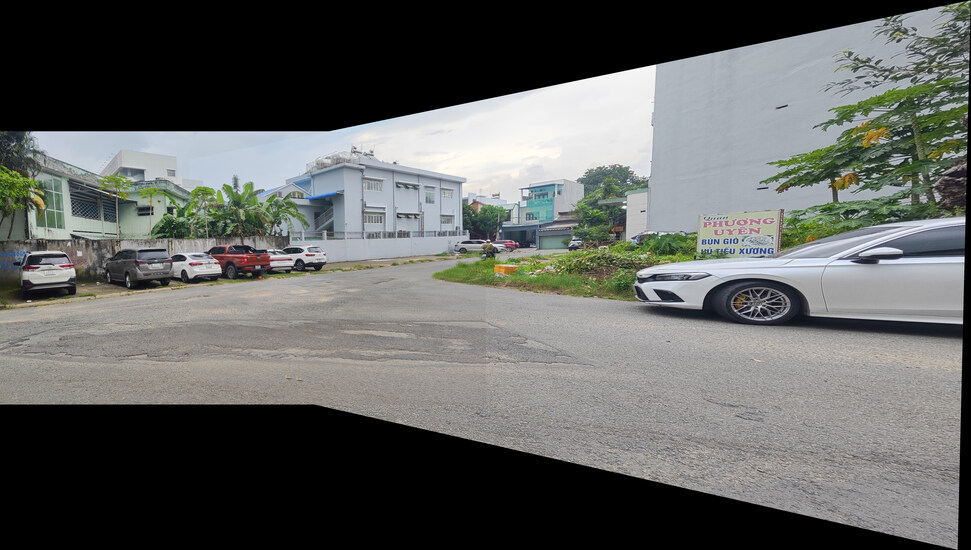
\includegraphics[width=\linewidth]{site2-large-panorama.jpg}
\caption{Ảnh panorama ghép từ cặp \texttt{site2/large} trong bộ ảnh Nhóm 16 (kết quả V4).}
\end{figure}
\end{columns}
\end{frame}

\begin{frame}{Sáu giai đoạn từ đặc trưng ảnh đến khung canvas}
\begin{figure}
\centering
\begin{tikzpicture}[
  stage/.style={draw=blue!60,fill=blue!7,rounded corners=2pt,align=center,
    minimum height=9mm,text width=2.75cm,font=\small}, node distance=5mm and 7mm,
  link/.style={-{Stealth[length=2mm]},thick}]
\node[stage] (s1) {S1 Tiền xử lý};
\node[stage,right=of s1] (s2) {S2 Keypoint};
\node[stage,right=of s2] (s3) {S3 Descriptor};
\node[stage,below=of s3] (s4) {S4 Matching};
\node[stage,left=of s4] (s5) {S5 Homography};
\node[stage,left=of s5] (s6) {S6 Warp \& hòa trộn};
\draw[link] (s1)--(s2); \draw[link] (s2)--(s3); \draw[link] (s3)--(s4);
\draw[link] (s4)--(s5); \draw[link] (s5)--(s6);
\end{tikzpicture}
\caption{Kiến trúc pipeline 6 giai đoạn từ tiền xử lý đến kết xuất panorama.}
\end{figure}

\begin{itemize}
\item S1--S3 xử lý độc lập trên từng ảnh A và B; S4--S6 kết hợp dữ liệu từ cả hai ảnh.
\item S1 chuyển ảnh xám và làm mượt Gaussian. S2 phát hiện góc FAST-9 (kèm NMS và chọn top-K), S3 tính descriptor BRIEF 256-bit.
\end{itemize}
\end{frame}

\begin{frame}{Khớp đặc trưng, ước lượng hình học và kết xuất}
\begin{itemize}
\item S4: Khớp descriptor nhị phân bằng khoảng cách Hamming (brute-force) và lọc cặp mơ hồ qua Lowe's ratio test.
\item S5: Lấy mẫu 4 cặp khớp cho mỗi giả thuyết MSAC RANSAC, chấm điểm homography ứng viên và khớp lại trên toàn bộ inlier (DLT + Jacobi SVD).
\item S6: Tính biên canvas, chiếu ngược pixel đầu ra về ảnh gốc, lấy mẫu bilinear trên B và hòa trộn vùng chồng lấn bằng trung bình 50/50.
\end{itemize}
\medskip
\small Homography giả định cảnh nằm trên một mặt phẳng hoặc camera chủ yếu xoay; hiệu ứng parallax mạnh hay hoa văn lặp vẫn có thể gây lỗi căn chỉnh.
\end{frame}

\begin{frame}{Một pipeline, sáu phiên bản (V0--V5)}
\begin{table}
\centering
\caption{Tóm tắt sáu phiên bản cài đặt của pipeline ghép ảnh (V0--V5).}
\begin{tabular}{lp{.71\linewidth}}
\toprule
Phiên bản & Thay đổi cài đặt chính \\
\midrule
V0 & Bản tuần tự CPU tham chiếu (đóng băng làm chuẩn). \\
V1 & CUDA cơ bản cho S1--S6 với bộ đệm trung gian device-resident. \\
V2 & Song song hóa chấm điểm RANSAC, rút gọn inlier và refit ở S5. \\
V3 & MSAC dùng warp-shuffle, DLT/SVD trên shared memory và chia batch ở S5. \\
V4 & Gộp kết xuất canvas một lượt ở S6 (bản production chính). \\
V5 & Thực thi bất đồng bộ hai CUDA stream cho H2D + S1--S3 (case study). \\
\bottomrule
\end{tabular}
\end{table}
\end{frame}

\section{Kiểm chứng, kết quả và phân tích hiệu năng}
\begin{frame}{Kiểm chứng độ chính xác và an toàn bộ nhớ}
\begin{itemize}
\item Đối chiếu từng stage: Mọi stage GPU đều được kiểm tra khớp với V0 trước khi tích hợp toàn pipeline.
\item Ảnh synthetic (6 cặp): RMSE $\le 0{,}10$ px và Max $\le 0{,}21$ px (ngưỡng: 0,5 / 1,0 px), độ lệch giữa các phiên bản bằng 0 px.
\item Bộ ảnh thật (12 cấu hình): Cả 10 ca hợp lệ khớp khung canvas V0 với Max RGB error = 0; \texttt{challenge/medium} và \texttt{large} giữ nguyên lỗi \texttt{NumericalFailure} ở S6.
\item An toàn bộ nhớ: \texttt{compute-sanitizer --tool memcheck --leak-check full} xác nhận 0 lỗi và 0 byte rò rỉ trên cả test suite GPU lẫn CLI.
\end{itemize}
\medskip
\small Nghiệm thu toàn bộ trên Tesla T4: 14 suite V0 (45.284 checks), 16 suite GPU cho V1--V5 (69.336 checks) và toàn bộ suite Python.
\end{frame}

\begin{frame}{Kết quả ảnh ghép và phân tích ca thất bại}
\begin{figure}
\centering
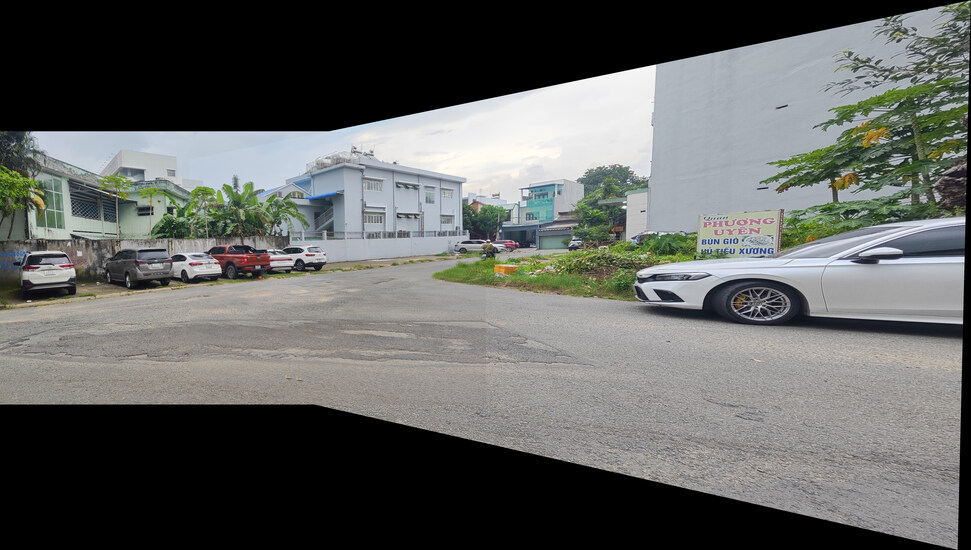
\includegraphics[width=.45\linewidth]{site2-large-panorama.jpg}
\caption{Cảnh ngoài trời hợp lệ \texttt{site2/large} (7676$\times$4348, kết quả V4).}
\end{figure}
\begin{itemize}
\item Ca thất bại (\texttt{challenge/medium}): Trả về \texttt{[NumericalFailure] S6 warp\_blend failed} nhất quán từ V0 đến V5.
\item Nguyên nhân gốc: Hoa văn lặp của lan can và trần nhà tạo ra nhiều cặp khớp BRIEF 256-bit mơ hồ, dẫn đến ma trận homography suy biến.
\end{itemize}
\end{frame}

% P9-T06: performance module by Le Thuong De (23120232).
% AI assistance: Codex helped draft and validate this module.
% Insert with % P9-T06: performance module by Le Thuong De (23120232).
% AI assistance: Codex helped draft and validate this module.
% Insert with % P9-T06: performance module by Le Thuong De (23120232).
% AI assistance: Codex helped draft and validate this module.
% Insert with \input{performance.tex} from the shared Beamer document.
\begin{frame}{How the experiment is controlled}
\begin{itemize}
\item One Tesla T4 session; one pinned source and binary for V0--V4.
\item Official dataset: 3 standard sites, 3 resolutions, plus challenge cases.
\item One warm-up and 5 measured runs per successful configuration.
\item Report stages, H2D, D2H, kernel total, and end-to-end separately.
\item Compare speedups only within the same measurement session.
\end{itemize}
\end{frame}

\begin{frame}{APOD: follow the measured bottleneck}
\begin{description}
\item[Assess] Identify the dominant stage using timing and Nsight.
\item[Parallelize] V1 moves the six-stage pipeline to CUDA.
\item[Optimize] V2/V3 target S5; V4 targets canvas construction in S6.
\item[Deploy] Preserve correctness, check memory safety, retain evidence.
\end{description}
\medskip
An improved stage can expose a different pipeline bottleneck.
\end{frame}

\begin{frame}{Why investigate S6 after V3?}
\centering
\begin{tabular}{lrr}
\toprule
P8, site2/large & V2 & V3 \\
\midrule
S5 (ms) & 30.538 & 12.200 \\
S6 (ms) & 29.580 & 28.468 \\
Pipeline total (ms) & 81.826 & 62.353 \\
\bottomrule
\end{tabular}
\medskip
\begin{itemize}
\item S6 accounts for 45.7\% of the V3 total in this historical run.
\item Even a 2$\times$ S6 speedup would allow only about 1.30$\times$ total speedup if everything else stayed constant.
\end{itemize}
\tiny Source: P8 report, 16 Nov 2026, same-session V2/V3; source checkout b3c79d7. Historical context only; P9 remeasures all versions.
\end{frame}

\begin{frame}{V4: single-pass canvas fusion}
\begin{block}{V3 renderer}
Clear canvas $\rightarrow$ copy A $\rightarrow$ gather and blend B.
\end{block}
\begin{block}{V4 renderer}
One thread per output pixel: test A/B validity, sample source pixels, blend, write RGB once.
\end{block}
\begin{itemize}
\item Keep canvas geometry, inverse projection, interpolation and rounding rules.
\item Reuse S1--S4 from V1 and S5 from V3.
\item Fewer passes suggest less traffic; hardware counters must verify actual DRAM traffic.
\end{itemize}
\end{frame}

\begin{frame}{Correctness before performance}
\begin{itemize}
\item P9-T02: six synthetic pairs and twelve real configurations on Tesla T4.
\item Accepted V4 source: \texttt{ab8df98d}; benchmark checks source equivalence.
\item Ten successful real cases: matching geometry and Max RGB = 0.
\item Challenge medium/large preserve the expected S6 NumericalFailure status.
\item Suite and production CLI memcheck: zero errors, zero bytes leaked.
\end{itemize}
\medskip
\tiny Source: docs/report/p9-v4-verification.md. Acceptance timing is excluded from benchmark tables.
\end{frame}

\begin{frame}{V4 benchmark: same-session comparison}
\input{generated/v4-table.tex}
\end{frame}

\begin{frame}{Nsight Systems shows three canvas operations become one}
\centering
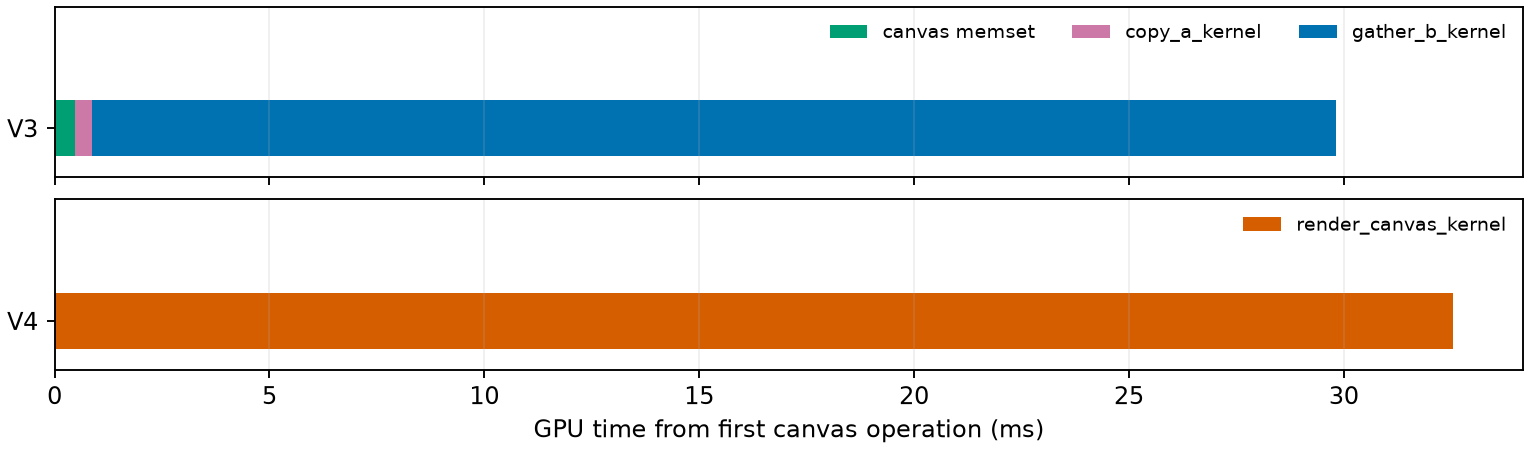
\includegraphics[width=.94\linewidth]{generated/nsys-v4.png}
\begin{itemize}
\item Tesla T4, site2/large, second pass of each trace.
\item V3 clear, copy A and gather B total 29.804 ms. V4 render takes 32.541 ms in this trace.
\item The five-run benchmark measures S6 at 28.712 ms for V3 and 28.190 ms for V4.
\end{itemize}
\end{frame}

\begin{frame}{Nsight Compute finds more DRAM traffic in sampled kernels}
\centering
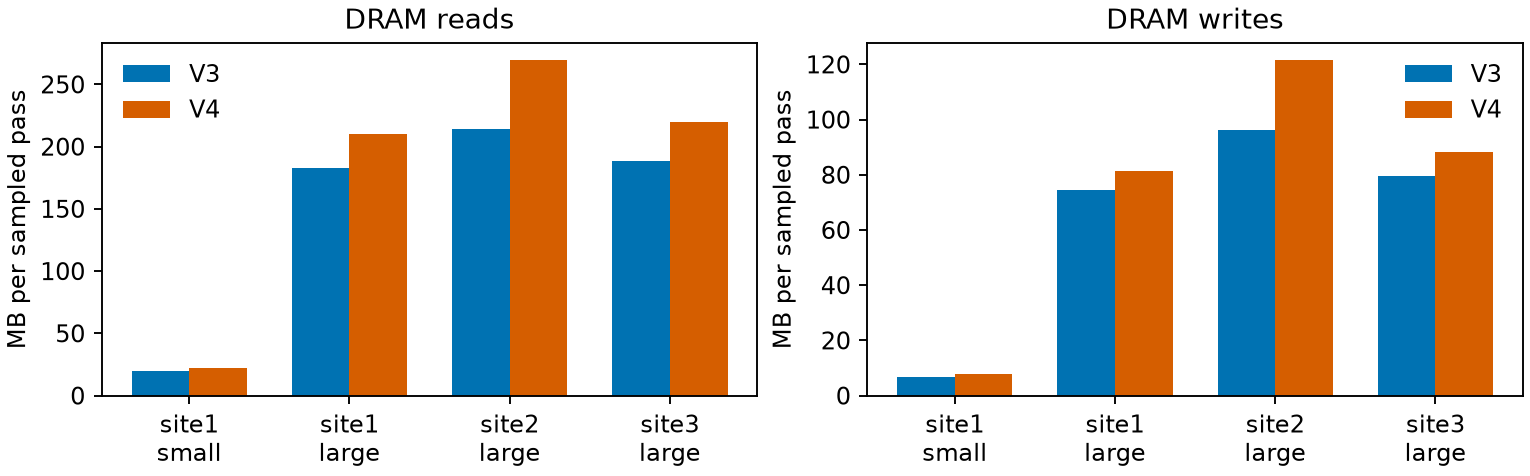
\includegraphics[width=.94\linewidth]{generated/ncu-v4.png}
\begin{itemize}
\item At site2/large, reads plus writes rise from 310.78 to 391.69 MB (+26.0\%).
\item The V3 bars sum one sample each of copy A and gather B. The V4 bars use one renderer sample. V3 canvas memset is outside the counter scope.
\end{itemize}
\end{frame}

\begin{frame}{What determines whether V4 is useful?}
\begin{itemize}
\item P9: V4 is faster in 8/9 standard cases; S6 geometric mean speedup is 1.0357$\times$.
\item Primary case paired blocks: median 1.0270$\times$, range 0.9774--1.0409$\times$; 4/5 blocks favor V4.
\item The primary case does not reach the previously proposed 5\% improvement threshold.
\item Keep challenge failures explicit; an absent timing is not zero time.
\item Separate profiler observations from unprofiled timing evidence.
\end{itemize}
\end{frame}

\begin{frame}{V5: dual-stream concurrency investigation}
\begin{block}{Two independent image branches}
Stream A and Stream B overlap H2D, S1, S2, and S3 concurrently; join before S4.
\end{block}
\begin{itemize}
\item Pre-S4 duration at site2/large decreases from $\sim$15.29 ms to $\sim$12.68 ms (1.207$\times$).
\item End-to-end speedup is modest (1.027$\times$ geometric mean) because downstream S5 and S6 dominate total time and SM resources are shared.
\item Confirms correctness and memory safety (0 memcheck errors, bit-for-bit parity with sequential mode).
\item Conclusion: V4 remains the production version; V5 serves as a concurrent stream case study.
\end{itemize}
\end{frame}

\begin{frame}{Lessons and limits}
\begin{itemize}
\item Faster S5 exposes S6; stage speedup is bounded by its pipeline share.
\item Fusion removes canvas passes. The sampled kernels show higher DRAM traffic.
\item Occupancy and throughput explain behavior; they are not the performance objective.
\item Preserve hashes, commands, raw runs, failures and original reports.
\item P9: total speedup is only 1.0086$\times$ (geometric mean); the benefit is modest.
\end{itemize}
\end{frame}
 from the shared Beamer document.
\begin{frame}{How the experiment is controlled}
\begin{itemize}
\item One Tesla T4 session; one pinned source and binary for V0--V4.
\item Official dataset: 3 standard sites, 3 resolutions, plus challenge cases.
\item One warm-up and 5 measured runs per successful configuration.
\item Report stages, H2D, D2H, kernel total, and end-to-end separately.
\item Compare speedups only within the same measurement session.
\end{itemize}
\end{frame}

\begin{frame}{APOD: follow the measured bottleneck}
\begin{description}
\item[Assess] Identify the dominant stage using timing and Nsight.
\item[Parallelize] V1 moves the six-stage pipeline to CUDA.
\item[Optimize] V2/V3 target S5; V4 targets canvas construction in S6.
\item[Deploy] Preserve correctness, check memory safety, retain evidence.
\end{description}
\medskip
An improved stage can expose a different pipeline bottleneck.
\end{frame}

\begin{frame}{Why investigate S6 after V3?}
\centering
\begin{tabular}{lrr}
\toprule
P8, site2/large & V2 & V3 \\
\midrule
S5 (ms) & 30.538 & 12.200 \\
S6 (ms) & 29.580 & 28.468 \\
Pipeline total (ms) & 81.826 & 62.353 \\
\bottomrule
\end{tabular}
\medskip
\begin{itemize}
\item S6 accounts for 45.7\% of the V3 total in this historical run.
\item Even a 2$\times$ S6 speedup would allow only about 1.30$\times$ total speedup if everything else stayed constant.
\end{itemize}
\tiny Source: P8 report, 16 Nov 2026, same-session V2/V3; source checkout b3c79d7. Historical context only; P9 remeasures all versions.
\end{frame}

\begin{frame}{V4: single-pass canvas fusion}
\begin{block}{V3 renderer}
Clear canvas $\rightarrow$ copy A $\rightarrow$ gather and blend B.
\end{block}
\begin{block}{V4 renderer}
One thread per output pixel: test A/B validity, sample source pixels, blend, write RGB once.
\end{block}
\begin{itemize}
\item Keep canvas geometry, inverse projection, interpolation and rounding rules.
\item Reuse S1--S4 from V1 and S5 from V3.
\item Fewer passes suggest less traffic; hardware counters must verify actual DRAM traffic.
\end{itemize}
\end{frame}

\begin{frame}{Correctness before performance}
\begin{itemize}
\item P9-T02: six synthetic pairs and twelve real configurations on Tesla T4.
\item Accepted V4 source: \texttt{ab8df98d}; benchmark checks source equivalence.
\item Ten successful real cases: matching geometry and Max RGB = 0.
\item Challenge medium/large preserve the expected S6 NumericalFailure status.
\item Suite and production CLI memcheck: zero errors, zero bytes leaked.
\end{itemize}
\medskip
\tiny Source: docs/report/p9-v4-verification.md. Acceptance timing is excluded from benchmark tables.
\end{frame}

\begin{frame}{V4 benchmark: same-session comparison}
% Generated from same-session P9 CSV; source ba97ed7, 2026-11-19.
\scriptsize
\centering
\begin{tabular}{llrrrr}
\toprule
Site & Size & V3 ms & V4 ms & Total speedup & S6 speedup \\
\midrule
site1 & small & 32.620 & 32.716 & 0.9971$\times$ & 1.0359$\times$ \\
site1 & medium & 31.027 & 30.785 & 1.0078$\times$ & 1.0633$\times$ \\
site1 & large & 108.107 & 107.157 & 1.0089$\times$ & 1.0061$\times$ \\
site2 & small & 21.415 & 21.142 & 1.0129$\times$ & 1.0368$\times$ \\
site2 & medium & 27.932 & 27.581 & 1.0127$\times$ & 1.0495$\times$ \\
site2 & large & 62.874 & 62.197 & 1.0109$\times$ & 1.0185$\times$ \\
site3 & small & 44.846 & 44.576 & 1.0061$\times$ & 1.0193$\times$ \\
site3 & medium & 56.167 & 55.723 & 1.0080$\times$ & 1.0403$\times$ \\
site3 & large & 101.713 & 100.393 & 1.0131$\times$ & 1.0525$\times$ \\
\bottomrule
\end{tabular}
\par\medskip Geometric mean total: 1.0086$\times$; S6: 1.0357$\times$.
\par One T4 session, one warm-up + 5 runs; nine standard cases.
\par\tiny Source: P9-T05, 19 Nov 2026, ba97ed7. Challenge failures excluded.

\end{frame}

\begin{frame}{Nsight Systems shows three canvas operations become one}
\centering
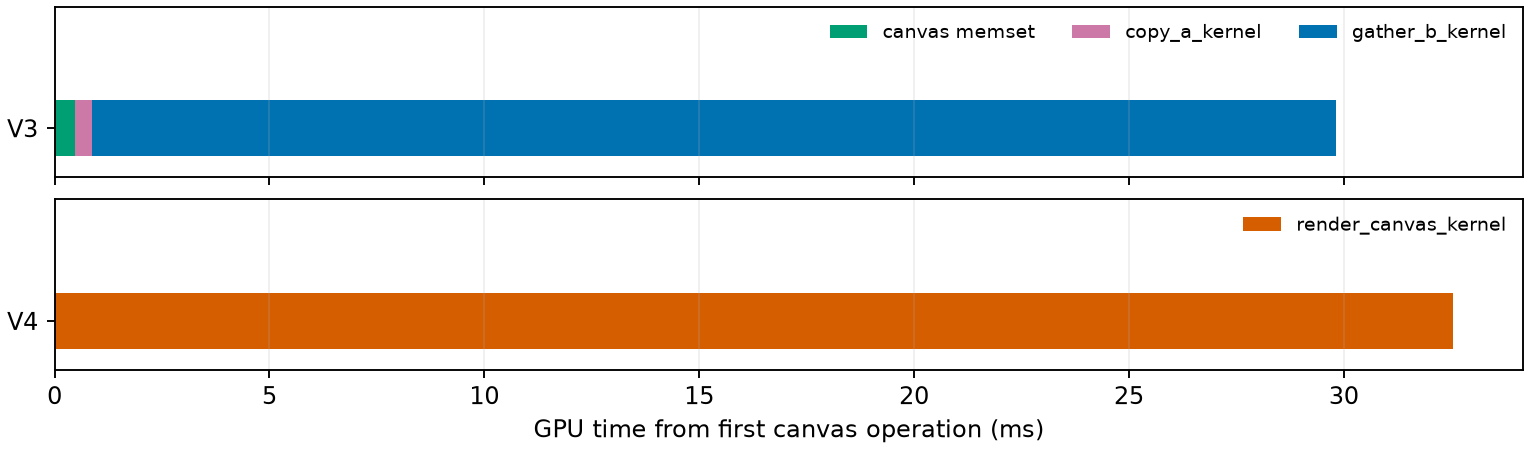
\includegraphics[width=.94\linewidth]{generated/nsys-v4.png}
\begin{itemize}
\item Tesla T4, site2/large, second pass of each trace.
\item V3 clear, copy A and gather B total 29.804 ms. V4 render takes 32.541 ms in this trace.
\item The five-run benchmark measures S6 at 28.712 ms for V3 and 28.190 ms for V4.
\end{itemize}
\end{frame}

\begin{frame}{Nsight Compute finds more DRAM traffic in sampled kernels}
\centering
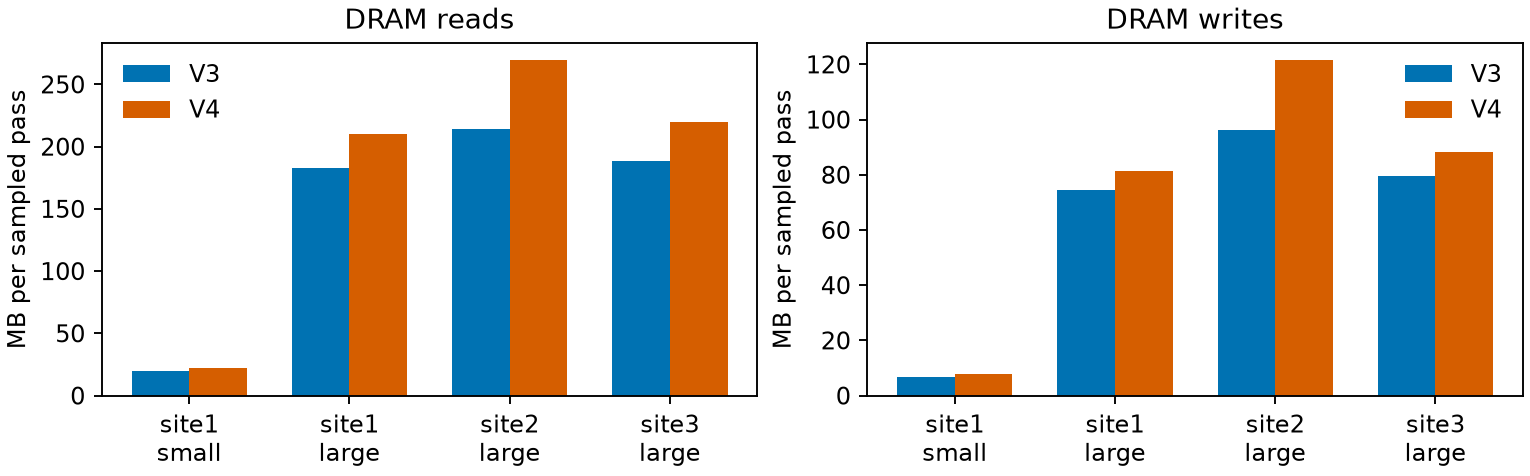
\includegraphics[width=.94\linewidth]{generated/ncu-v4.png}
\begin{itemize}
\item At site2/large, reads plus writes rise from 310.78 to 391.69 MB (+26.0\%).
\item The V3 bars sum one sample each of copy A and gather B. The V4 bars use one renderer sample. V3 canvas memset is outside the counter scope.
\end{itemize}
\end{frame}

\begin{frame}{What determines whether V4 is useful?}
\begin{itemize}
\item P9: V4 is faster in 8/9 standard cases; S6 geometric mean speedup is 1.0357$\times$.
\item Primary case paired blocks: median 1.0270$\times$, range 0.9774--1.0409$\times$; 4/5 blocks favor V4.
\item The primary case does not reach the previously proposed 5\% improvement threshold.
\item Keep challenge failures explicit; an absent timing is not zero time.
\item Separate profiler observations from unprofiled timing evidence.
\end{itemize}
\end{frame}

\begin{frame}{V5: dual-stream concurrency investigation}
\begin{block}{Two independent image branches}
Stream A and Stream B overlap H2D, S1, S2, and S3 concurrently; join before S4.
\end{block}
\begin{itemize}
\item Pre-S4 duration at site2/large decreases from $\sim$15.29 ms to $\sim$12.68 ms (1.207$\times$).
\item End-to-end speedup is modest (1.027$\times$ geometric mean) because downstream S5 and S6 dominate total time and SM resources are shared.
\item Confirms correctness and memory safety (0 memcheck errors, bit-for-bit parity with sequential mode).
\item Conclusion: V4 remains the production version; V5 serves as a concurrent stream case study.
\end{itemize}
\end{frame}

\begin{frame}{Lessons and limits}
\begin{itemize}
\item Faster S5 exposes S6; stage speedup is bounded by its pipeline share.
\item Fusion removes canvas passes. The sampled kernels show higher DRAM traffic.
\item Occupancy and throughput explain behavior; they are not the performance objective.
\item Preserve hashes, commands, raw runs, failures and original reports.
\item P9: total speedup is only 1.0086$\times$ (geometric mean); the benefit is modest.
\end{itemize}
\end{frame}
 from the shared Beamer document.
\begin{frame}{How the experiment is controlled}
\begin{itemize}
\item One Tesla T4 session; one pinned source and binary for V0--V4.
\item Official dataset: 3 standard sites, 3 resolutions, plus challenge cases.
\item One warm-up and 5 measured runs per successful configuration.
\item Report stages, H2D, D2H, kernel total, and end-to-end separately.
\item Compare speedups only within the same measurement session.
\end{itemize}
\end{frame}

\begin{frame}{APOD: follow the measured bottleneck}
\begin{description}
\item[Assess] Identify the dominant stage using timing and Nsight.
\item[Parallelize] V1 moves the six-stage pipeline to CUDA.
\item[Optimize] V2/V3 target S5; V4 targets canvas construction in S6.
\item[Deploy] Preserve correctness, check memory safety, retain evidence.
\end{description}
\medskip
An improved stage can expose a different pipeline bottleneck.
\end{frame}

\begin{frame}{Why investigate S6 after V3?}
\centering
\begin{tabular}{lrr}
\toprule
P8, site2/large & V2 & V3 \\
\midrule
S5 (ms) & 30.538 & 12.200 \\
S6 (ms) & 29.580 & 28.468 \\
Pipeline total (ms) & 81.826 & 62.353 \\
\bottomrule
\end{tabular}
\medskip
\begin{itemize}
\item S6 accounts for 45.7\% of the V3 total in this historical run.
\item Even a 2$\times$ S6 speedup would allow only about 1.30$\times$ total speedup if everything else stayed constant.
\end{itemize}
\tiny Source: P8 report, 16 Nov 2026, same-session V2/V3; source checkout b3c79d7. Historical context only; P9 remeasures all versions.
\end{frame}

\begin{frame}{V4: single-pass canvas fusion}
\begin{block}{V3 renderer}
Clear canvas $\rightarrow$ copy A $\rightarrow$ gather and blend B.
\end{block}
\begin{block}{V4 renderer}
One thread per output pixel: test A/B validity, sample source pixels, blend, write RGB once.
\end{block}
\begin{itemize}
\item Keep canvas geometry, inverse projection, interpolation and rounding rules.
\item Reuse S1--S4 from V1 and S5 from V3.
\item Fewer passes suggest less traffic; hardware counters must verify actual DRAM traffic.
\end{itemize}
\end{frame}

\begin{frame}{Correctness before performance}
\begin{itemize}
\item P9-T02: six synthetic pairs and twelve real configurations on Tesla T4.
\item Accepted V4 source: \texttt{ab8df98d}; benchmark checks source equivalence.
\item Ten successful real cases: matching geometry and Max RGB = 0.
\item Challenge medium/large preserve the expected S6 NumericalFailure status.
\item Suite and production CLI memcheck: zero errors, zero bytes leaked.
\end{itemize}
\medskip
\tiny Source: docs/report/p9-v4-verification.md. Acceptance timing is excluded from benchmark tables.
\end{frame}

\begin{frame}{V4 benchmark: same-session comparison}
% Generated from same-session P9 CSV; source ba97ed7, 2026-11-19.
\scriptsize
\centering
\begin{tabular}{llrrrr}
\toprule
Site & Size & V3 ms & V4 ms & Total speedup & S6 speedup \\
\midrule
site1 & small & 32.620 & 32.716 & 0.9971$\times$ & 1.0359$\times$ \\
site1 & medium & 31.027 & 30.785 & 1.0078$\times$ & 1.0633$\times$ \\
site1 & large & 108.107 & 107.157 & 1.0089$\times$ & 1.0061$\times$ \\
site2 & small & 21.415 & 21.142 & 1.0129$\times$ & 1.0368$\times$ \\
site2 & medium & 27.932 & 27.581 & 1.0127$\times$ & 1.0495$\times$ \\
site2 & large & 62.874 & 62.197 & 1.0109$\times$ & 1.0185$\times$ \\
site3 & small & 44.846 & 44.576 & 1.0061$\times$ & 1.0193$\times$ \\
site3 & medium & 56.167 & 55.723 & 1.0080$\times$ & 1.0403$\times$ \\
site3 & large & 101.713 & 100.393 & 1.0131$\times$ & 1.0525$\times$ \\
\bottomrule
\end{tabular}
\par\medskip Geometric mean total: 1.0086$\times$; S6: 1.0357$\times$.
\par One T4 session, one warm-up + 5 runs; nine standard cases.
\par\tiny Source: P9-T05, 19 Nov 2026, ba97ed7. Challenge failures excluded.

\end{frame}

\begin{frame}{Nsight Systems shows three canvas operations become one}
\centering
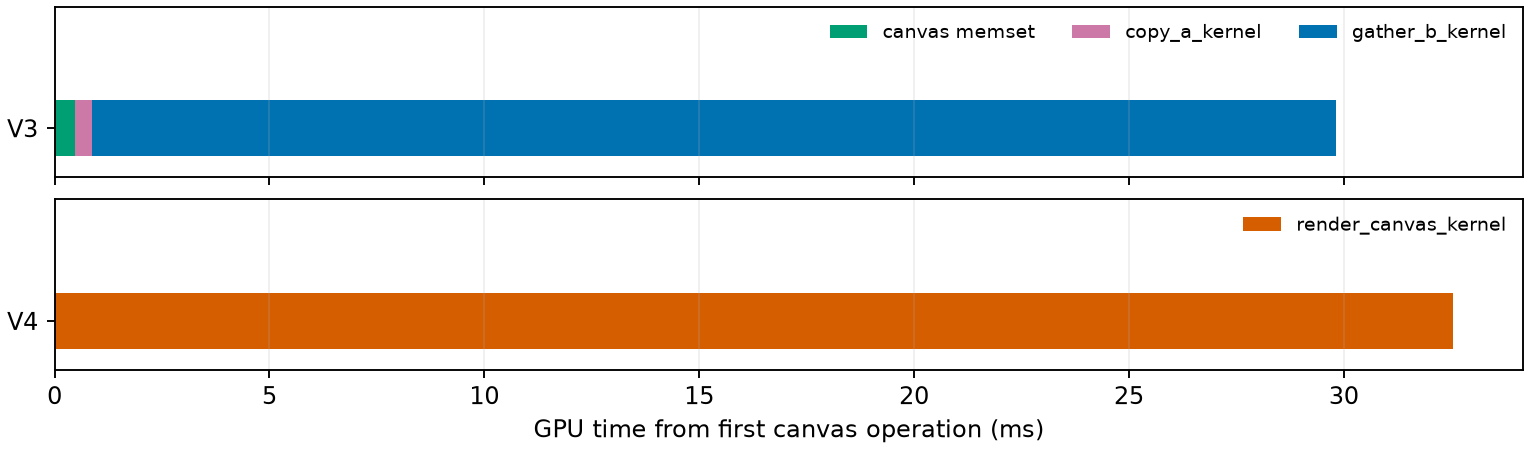
\includegraphics[width=.94\linewidth]{generated/nsys-v4.png}
\begin{itemize}
\item Tesla T4, site2/large, second pass of each trace.
\item V3 clear, copy A and gather B total 29.804 ms. V4 render takes 32.541 ms in this trace.
\item The five-run benchmark measures S6 at 28.712 ms for V3 and 28.190 ms for V4.
\end{itemize}
\end{frame}

\begin{frame}{Nsight Compute finds more DRAM traffic in sampled kernels}
\centering
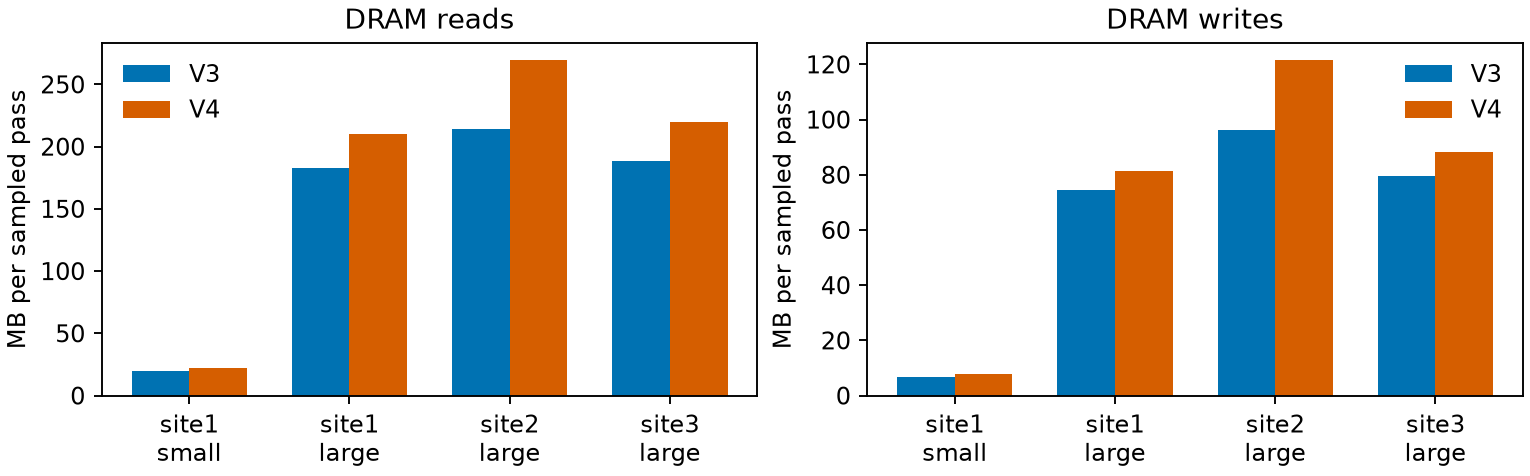
\includegraphics[width=.94\linewidth]{generated/ncu-v4.png}
\begin{itemize}
\item At site2/large, reads plus writes rise from 310.78 to 391.69 MB (+26.0\%).
\item The V3 bars sum one sample each of copy A and gather B. The V4 bars use one renderer sample. V3 canvas memset is outside the counter scope.
\end{itemize}
\end{frame}

\begin{frame}{What determines whether V4 is useful?}
\begin{itemize}
\item P9: V4 is faster in 8/9 standard cases; S6 geometric mean speedup is 1.0357$\times$.
\item Primary case paired blocks: median 1.0270$\times$, range 0.9774--1.0409$\times$; 4/5 blocks favor V4.
\item The primary case does not reach the previously proposed 5\% improvement threshold.
\item Keep challenge failures explicit; an absent timing is not zero time.
\item Separate profiler observations from unprofiled timing evidence.
\end{itemize}
\end{frame}

\begin{frame}{V5: dual-stream concurrency investigation}
\begin{block}{Two independent image branches}
Stream A and Stream B overlap H2D, S1, S2, and S3 concurrently; join before S4.
\end{block}
\begin{itemize}
\item Pre-S4 duration at site2/large decreases from $\sim$15.29 ms to $\sim$12.68 ms (1.207$\times$).
\item End-to-end speedup is modest (1.027$\times$ geometric mean) because downstream S5 and S6 dominate total time and SM resources are shared.
\item Confirms correctness and memory safety (0 memcheck errors, bit-for-bit parity with sequential mode).
\item Conclusion: V4 remains the production version; V5 serves as a concurrent stream case study.
\end{itemize}
\end{frame}

\begin{frame}{Lessons and limits}
\begin{itemize}
\item Faster S5 exposes S6; stage speedup is bounded by its pipeline share.
\item Fusion removes canvas passes. The sampled kernels show higher DRAM traffic.
\item Occupancy and throughput explain behavior; they are not the performance objective.
\item Preserve hashes, commands, raw runs, failures and original reports.
\item P9: total speedup is only 1.0086$\times$ (geometric mean); the benefit is modest.
\end{itemize}
\end{frame}


\section{Các tối ưu chính và bài học rút ra}
\begin{frame}{Chu trình APOD: tối ưu theo điểm nghẽn đo được}
\begin{itemize}
\item Assess: Đo thời gian từng stage và phân tích trace Nsight Systems / Compute.
\item Parallelize: V1 chuyển S1--S6 lên CUDA với bộ nhớ device-resident để bỏ sao chép H2D/D2H trung gian.
\item Optimize: V2/V3 tăng tốc S5; V4 gộp các lượt ghi canvas ở S6; V5 chồng lấp H2D + S1--S3 trên hai CUDA stream.
\item Deploy: Kiểm chứng tương đương đầu ra và an toàn bộ nhớ trước khi chấp nhận mỗi tối ưu.
\end{itemize}
\medskip
Mỗi bước tối ưu làm lộ diện điểm nghẽn kế tiếp, cho đến khi định luật Amdahl giới hạn mức tăng tốc toàn pipeline.
\end{frame}

\begin{frame}{Tối ưu S5 (V2 \& V3): giải quyết điểm nghẽn 90\%+}
\begin{itemize}
\item Vì sao chọn S5 trước? Ở V1, RANSAC tuần tự trên GPU chiếm 90--99\% tổng thời gian trên cả 9 ca chuẩn.
\item V2 (RANSAC song song): Đánh giá song song các giả thuyết, song song hóa rút gọn inlier và đưa bước refit cuối lên GPU $\rightarrow$ nhanh hơn V1 6,16$\times$ (23,4$\times$ so với V0).
\item V3 (Tối ưu vi kiến trúc):
  \begin{itemize}
  \item Chấm điểm MSAC bằng warp-shuffle giúp giảm chi phí shared memory và đồng bộ.
  \item DLT 4 điểm / Jacobi SVD trên shared memory kèm chia batch để tăng độ khai thác SM.
  \end{itemize}
\item Hiệu quả: Tăng thêm 1,83$\times$ toàn pipeline (42,7$\times$ so với V0), kéo S5 trên \texttt{site2/large} xuống 12,2 ms và làm S6 trở thành điểm nghẽn mới.
\end{itemize}
\end{frame}

\begin{frame}{Tối ưu V4: gộp kết xuất canvas trong một lượt}
\begin{itemize}
\item Bộ kết xuất V3 (3 lượt): Xóa canvas (\texttt{cudaMemset}) $\rightarrow$ sao chép ảnh A $\rightarrow$ lấy mẫu và hòa trộn ảnh B.
\item Bộ kết xuất V4 (1 lượt gộp): Mỗi thread xử lý một pixel đầu ra: kiểm tra biên A/B, lấy mẫu ảnh gốc, hòa trộn 50/50 và ghi RGB một lần.
\item Giữ nguyên khung canvas, phép chiếu ngược, nội suy bilinear và quy tắc làm tròn (Max RGB error = 0); tái sử dụng S1--S4 (V1) và S5 (V3).
\item Nhanh hơn ở 8/9 ca chuẩn (S6 GM 1,04$\times$, tổng GM 1,01$\times$; 4/5 khối ghép cặp trên \texttt{site2/large} nghiêng về V4, trung vị 1,03$\times$).
\item Đánh đổi: Bỏ được hai lượt ghi canvas nhưng Nsight Compute cho thấy lưu lượng DRAM tăng, giới hạn speedup tổng quanh $\sim$1\%.
\end{itemize}
\end{frame}

\begin{frame}{Tối ưu V5: xử lý song song bằng hai CUDA stream}
\begin{itemize}
\item Động lực: Sau V4, phần tiền S4 (H2D + S1--S3 của hai ảnh) chiếm 11,2\% (\texttt{site3/large}), 12,2\% (\texttt{site1/large}) và 21,4\% (\texttt{site2/large}, 15,3 ms) tổng thời gian.
\item Chạy ảnh A và B trên hai CUDA stream không chặn (\texttt{streamA}, \texttt{streamB}) với scratch buffer tách biệt và pinned memory cho bộ đếm ứng viên.
\item Lập lịch prefix/suffix: Đẩy H2D + S1 + ứng viên S2 trên cả hai nhánh, thăm dò \texttt{cudaEventQuery} kèm \texttt{yield()}, rồi chạy S2 top-K + S3 cho nhánh xong trước.
\item Stream điều phối chờ \texttt{doneA}/\texttt{doneB} bằng \texttt{cudaStreamWaitEvent}, gộp bộ đếm rồi chạy S4--S6.
\item Tích hợp cờ đối chứng (\texttt{--v5-schedule sequential}) để tách riêng tác dụng đồng thời của stream khỏi thay đổi bố cục bộ nhớ.
\end{itemize}
\end{frame}

\begin{frame}{Bài học rút ra và giới hạn hiện tại}
\begin{itemize}
\item Bám sát số đo và định luật Amdahl: Xử lý S5 mang lại phần lớn mức tăng tốc (42,7$\times$); các tối ưu sau ở S6 (45,7\%) và tiền S4 (21,4\%) bị giới hạn trần chặt hơn nhiều.
\item Chỉ số phần cứng chính xác hơn trực giác: Gộp ba lượt S6 tưởng như tiết kiệm băng thông, nhưng Nsight Compute chỉ ra lưu lượng DRAM tăng +26\% và L2 hit rate giảm trên \texttt{site2/large}.
\item Xử lý đồng thời chịu giới hạn phần cứng: Hai stream đạt 17--25\% chồng lấp GPU và tăng tốc tiền S4 1,26$\times$, nhưng bão hòa SM trên Tesla T4 cùng +64,3 MiB VRAM khiến V4 ổn định hơn cho bản production.
\item Kiểm chứng trước khi đo đạc: So khớp chặt (Max RGB = 0), xử lý lỗi rõ ràng và memcheck bảo đảm mọi con số speedup đều đến từ pipeline đúng và không rò rỉ bộ nhớ.
\end{itemize}
\medskip
\small Toàn bộ kết quả có thể tái lập từ \texttt{Group16\_Final.ipynb}, file CSV gốc và trace Nsight trên Google Colab Tesla T4.
\end{frame}

\begin{frame}{Tài liệu tham khảo}
\scriptsize
\begin{itemize}
\item ITU-R Recommendation BT.601-7 (2011). Studio encoding parameters of digital television (hệ số chuyển ảnh xám S1).
\item Rosten, E. \& Drummond, T. (2006). Machine learning for high-speed corner detection, ECCV (thuật toán góc FAST-9 ở S2).
\item Calonder, M., Lepetit, V., Strecha, C., \& Fua, P. (2010). BRIEF: Binary Robust Independent Elementary Features, ECCV (descriptor nhị phân 256-bit ở S3).
\item Lowe, D. G. (2004). Distinctive Image Features from Scale-Invariant Keypoints, IJCV 60(2), 91--110 (Lowe's ratio test ở S4).
\item Brown, M. \& Lowe, D. G. (2007). Automatic Panoramic Image Stitching using Invariant Features, IJCV 74, 59--73 (RANSAC, DLT và hòa trộn ảnh).
\item Drmač, Z. \& Veselić, K. (2008). New Fast and Accurate Jacobi SVD Algorithm: II, LAPACK Working Note 170 (Jacobi SVD cho DLT ở S5).
\item Szeliski, R. (2006). Image Alignment and Stitching: A Tutorial, Foundations and Trends in Computer Graphics and Vision 2(1) (hệ quy chiếu, nội suy và kết xuất canvas ở S6).
\item NVIDIA (2025). CUDA C++ Best Practices Guide 13.0, Nsight Systems User Guide, Nsight Compute CLI và NVTX v3.
\end{itemize}
\end{frame}
\end{document}
